\documentclass[11pt]{article}
\usepackage{amsmath, amssymb, amsthm}
\usepackage{geometry}
\usepackage{graphicx}
\geometry{margin=1in}
\title{Foundations of Machine Learning -- Lecture 6 Notes}
\author{}
\date{}

\begin{document}
\maketitle

\section*{Classification Metrics}

\begin{figure}[h]
	\centering
	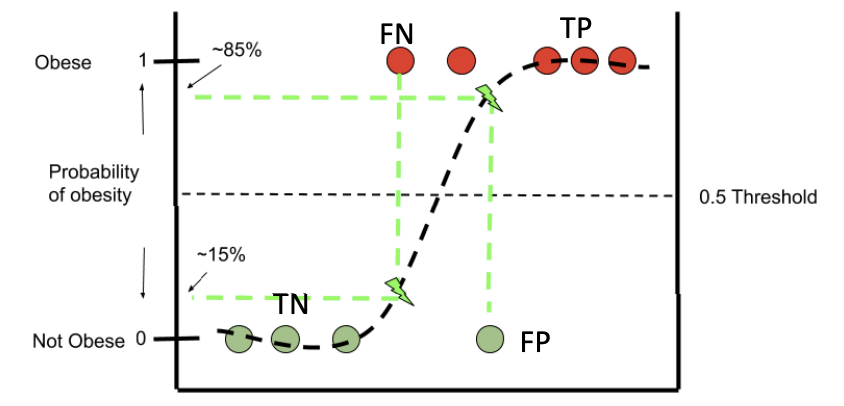
\includegraphics[width=0.6\textwidth]{../imgs/tnfn.png} % 
	\caption{Threshold results}
\end{figure}

\begin{itemize}
	\item \textbf{True Positive:} We predicted positive and it's positive.
	\item \textbf{True Negative:} We predicted negative and it's negative.
	\item \textbf{False Positive (Type 1 Error):} We predicted positive and it's negative.
	\item \textbf{False Negative (Type 2 Error):} We predicted negative and it's positive.
\end{itemize}

\paragraph*{Accuracy}
How often the classifier correctly predicts
\[
	\text{Accuracy} = \frac{TP + TN}{TP + TN + FP + FN}
\]
Good when classes are balanced but can be misleading when target class is sparse.
\paragraph*{Example}
We have a dataset with 10 positive samples (FN)
and 1000 of negative samples (TN). The Model classifies everything as negative.
This results in a misleading accuracy of \textbf{99\%}%

\paragraph*{Precision}
How many of the positive predicted cases actually turn out to be positive
\[
	\text{Precision} = \frac{TP}{TP+FP}
\]
Good when we want to be certain that our predicted positives are indeed positives,
but does not care about false negatives.

\paragraph*{Recall}
How many of the actual positive cases we were able
to predict correctly with our model.
\[
	\text{Recall} = \frac{TP}{TP + FN}
\]
Good when we want to capture all positives, does not care about false positives.

\paragraph*{F1-Score}
Harmonic mean of precision and recall
\[
	F_1 = 2\frac{Precision \cdot Recall}{Precision + Recall}
\]
Good when we want to have a model with both precision and recall. Bad if you only care about precision or recall and not both.
Gives equal weight to precision and recall.


\paragraph*{$F_\beta$-Score}
Weighted harmonic mean of precision and recall
\[
	F_\beta = (1+\beta^2)\frac{Precision \cdot Recall}{(\beta^2 \cdot Precision) + Recall}
\]


\paragraph*{ROC Curve}
This a visual representation of model performance across all thresholds
The ROC curve is drawn by calculating the true positive rate (TPR) and the false positive rate (FPR)
across threshold intervals.
\[
	\text{True positive rate (Recall)} = \frac{TP}{TP+FN}
\]
How many correct positive results occur among all positive samples

\[
	\text{False positive rate} = \frac{FP}{FP+TN}
\]
How many incorrect positive results occur among all negative samples


\begin{figure}[h]
	\centering
	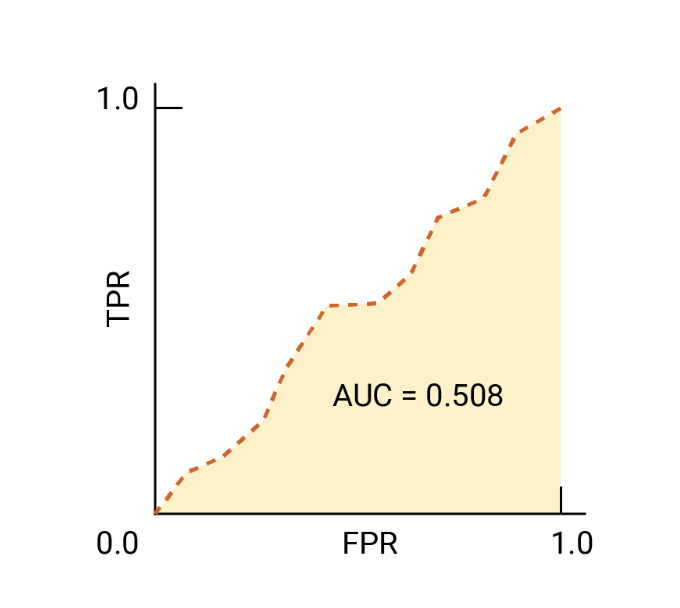
\includegraphics[width=0.35\textwidth]{../imgs/auc.png} % 
	\caption{Example ROC Curve}
\end{figure}

\begin{figure}[h]
	\centering
	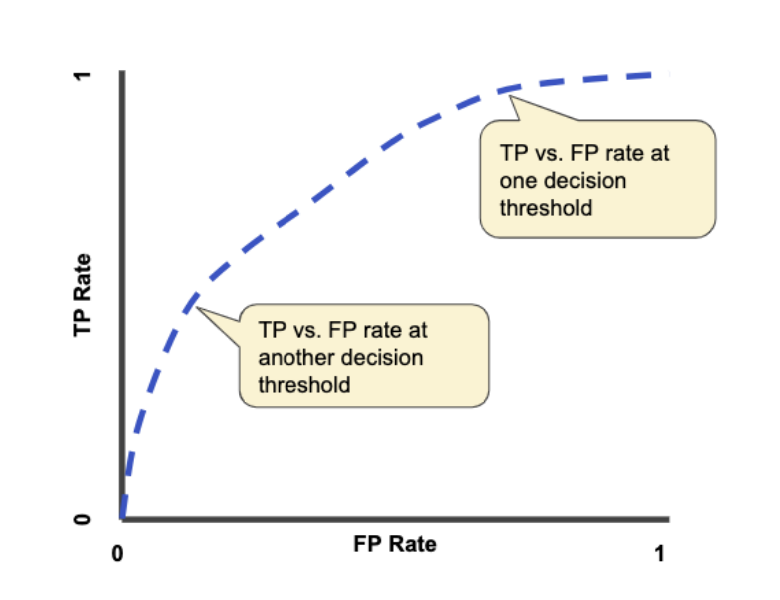
\includegraphics[width=0.35\textwidth]{../imgs/roc.png} % 
	\caption{Example ROC Curve}
\end{figure}

\textbf{AUC:} Area Under the ROC Curve, this provides an aggregate measure of performance across all possible classification thresholds.

\end{document}

